\documentclass{beamer}

\mode<presentation>
{
  \usetheme{Darmstadt}      % or try Darmstadt, Madrid, Warsaw, ...
  \usecolortheme{default} % or try albatross, beaver, crane, ...
  \usefonttheme{serif}  % or try serif, structurebold, ...
  \setbeamertemplate{navigation symbols}{}
  \setbeamertemplate{caption}[numbered]
} 
 
\usepackage[utf8]{inputenc}
\usepackage[]{algorithm2e}

%Information to be included in the title page:
\title{Scientific Analysis for:
Editing of Pig DNA May Lead to More Organs for People}
\author{Youngduck Choi, Amy Jung, Vaughn Tajirian, Katie Westerlund }
\institute{CILVR Lab, New York University}
 
\begin{document}
 
\frame{\titlepage}
 
\begin{frame}
\frametitle{Motivation}
\begin{itemize}
An

\bigskip

\item The applicability of deep learning, however, is not yet comprehensive.  

\bigskip

\item Can we get a state-of-the-art result for a well defined supervised task in medical domain
using deep learning?
\end{itemize}
\end{frame}

\begin{frame}
\frametitle{Problem: Early Detection of Diabetes from Claims}
\begin{figure}[htb]
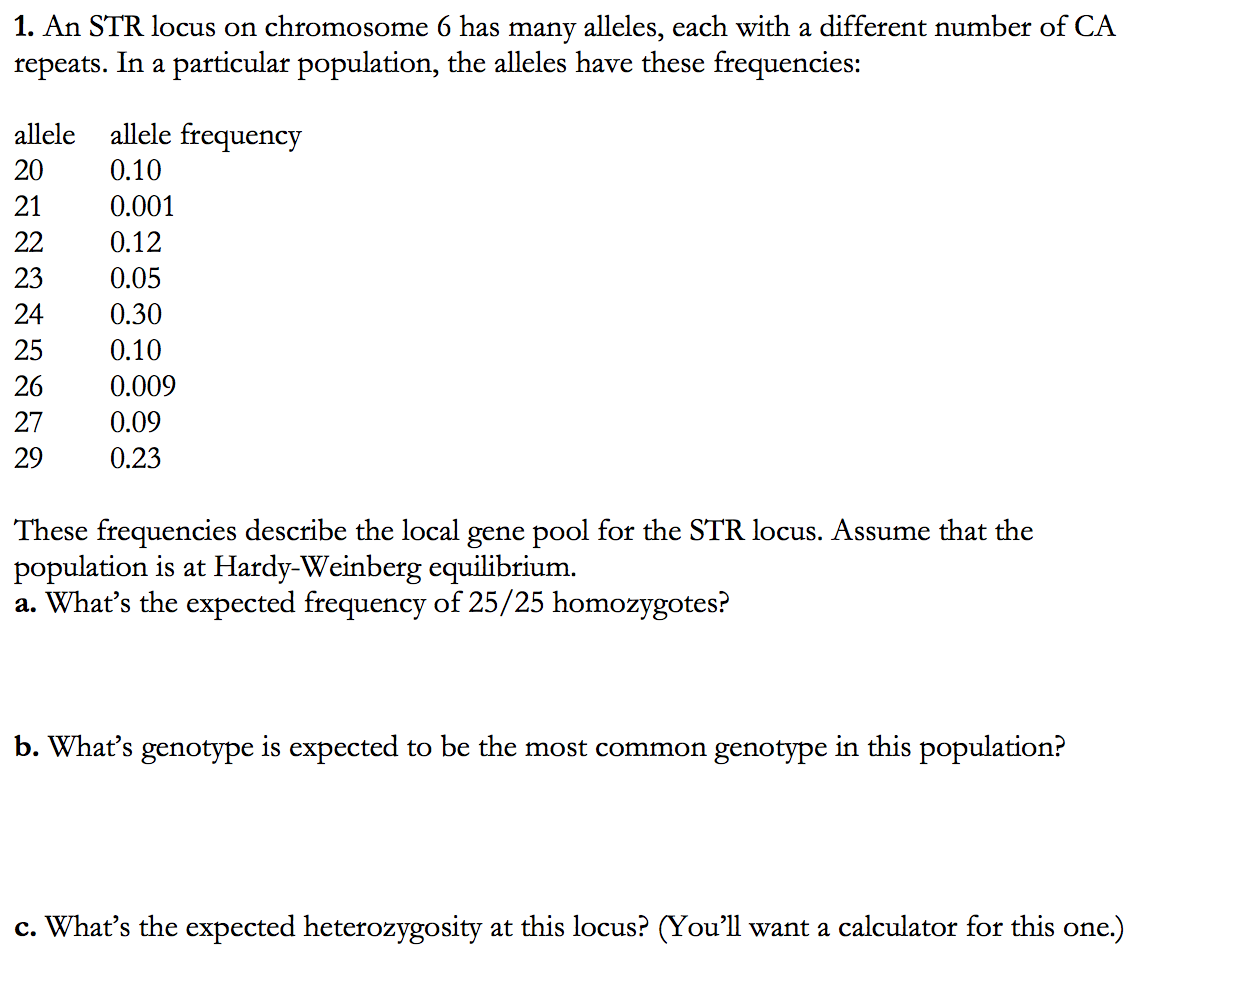
\includegraphics[width=0.7\textwidth]{genetics-9-1.png}
\caption{Various supervised tasks}
\end{figure} 
\end{frame}

\begin{frame}
\frametitle{Neighbors I}
\begin{figure}[htb]
Top 50 cosine distance codes: \\
4394155 (religious affiliation) : 1.0 \\
4319594 (sufficiency of income for needs) : 0.886792323995 \\
4320469 (low motivation) : 0.875451444993 \\
4419678 (auditory and visual hallucinations) : 0.861213899833 \\
4276205 (inability to cope) : 0.860558423511 \\
4864857 (poor cognition) : 0.860319009683 \\
4548639 (morphine 20 mg) : 0.858606201488 \\
4122208 (swearing) : 0.858280502692 \\
4247373 (fidgeting) : 0.855690125451 \\
4121999 (labile affect) : 0.855292082459 \\
4311835 (incoherent) : 0.854193874673 \\
4528103 (morphine 20 mg/ml oral solution) : 0.850018284495 \\
4120301 (moderate anxiety) : 0.849993724872 \\
\end{figure}
\end{frame}

\begin{frame}
\frametitle{Neighbors II}
\begin{figure}[htb]
Top 50 cosine distance codes: \\
4000978 (alzheimer's disease) : 1.0 \\
4305675 (aricept) : 0.927681307567 \\
4749486 (alzheimer's disease pathway kegg) : 0.90958817619 \\
4305676 (donepezil) : 0.906635582954 \\
4656147 (namenda) : 0.903731091715 \\
4298078 (dementia) : 0.884320489297 \\
4012831 (memantine) : 0.883449173077 \\
4005600 (presenile dementia) : 0.864689763427 \\
4605035 (mild cognitive disorder) : 0.859568216842 \\
4183905 (infarction, lacunar) : 0.847736673577 \\
4464452 (demented) : 0.836936999719 \\
\end{figure}
\end{frame}


\begin{frame}
\frametitle{Defining the Surrogate Measures for Embedding Space Properties}
\begin{itemize}
\item NDR-RT relation rank statistics score : let $(x,y)$ be a pair that encodes certain medical relationship
z(i.e. may treat). We say that if the embedded structure has the entity y as in the neighborhood of
x where the neighborhood of x is defined as
the top-k entities that are sorted by the inner product score with respect to x,
then it exhibits "relatedness" with respect to z.
\end{itemize}
\end{frame}
\begin{frame}
\frametitle{Defining the Surrogate Measures for Embedding Space Properties}
\begin{itemize}
\item
UMLS semantic type rank statistics score: let (x,t) be a pair of medical entity x with type t.
We say that if the embedded structure has an entity y of same type t in the neighborhood of x where the neighborhood of x is defined as the top-k entities that are sorted by the inner product score with respect to x, then it exhibits 'conceptual similarity."
\end{itemize}
\end{frame}


\begin{frame}
\frametitle{UMLS Semantic Type Scoring System}
\begin{footnotesize}
\begin{figure}[htb]
4003436 (carcinoma, non-small-cell lung, C0007131,  ['Neoplastic Process']) : 1.0 \\
4069419 (small cell carcinoma of lung, C0149925,  ['Neoplastic Process']) : 0.955599426233 \\
4394316 (carcinoma of lung, C0684249,  ['Neoplastic Process']) : 0.933888909808 \\
4125384 (malignant neoplasm of lung, C0242379,  ['Neoplastic Process']) : 0.928970432186 \\
4070138 (adenocarcinoma of lung (disorder), C0152013,  ['Neoplastic Process']) : 0.924754262378 \\
4555365 (tarceva, C1135136,  ['Organic Chemical', 'Pharmacologic Substance']) : 0.917757636841 \\
4069342 (lung mass, C0149726,  ['Finding']) : 0.914073299934 \\
\end{figure}
\end{footnotesize}
\end{frame}


\begin{frame}
\frametitle{Empirical Result I}
\begin{table}[t]
\begin{center}
\caption{Neighbor and Analogy Results on the May Treat Relationship. 
    Total 722 drugs were queried.}
\label{may_treat}
\begin{small}
\begin{sc}
\resizebox{8.2cm}{!}{
\begin{tabular}{|c|c|c|c|}
    \hline
                      & neighbors & analogy mean & analogy max \\
    \hline
    MedCopora           & 9.8338\% & 21.7299\% & 41.4127\% \\
    \hline
    10Bil,30d,s500,ns20 & 27.7008\% & 20.2710\% & 43.9058\% \\
    \hline
    10Bil,30d,s300,ns20 & 28.5319\% & 20.4457\% & 42.6593\% \\
    \hline
    10Bil,30d,s400,ns50 & {\bf 30.7479\%} & 25.6753\% & 45.7064\% \\
    \hline
    1Bil,1d,s300,ns20   & 30.6094\% & 25.4884\% & {\bf 47.6454\%} \\
    \hline
    1Bil,7d,s300,ns20   & 30.3324\% & 24.9829\% & 46.2604\% \\
    \hline
    svd,s100,ns10       & 31.4404\% & 18.7605\% & 31.7175\% \\
    \hline
    svd,s300,ns10       & 35.4571\% & 22.8062\% & 41.1357\% \\
    \hline
    svd,s500,ns10       & 39.1967\% & 24.6856\% & 42.2438\% \\
    \hline
    svd,s1000,ns10      & 42.9363\% & 26.8280\% & 43.6288\% \\
    \hline
\end{tabular}
}
\end{sc}
\end{small}
\end{center}
\end{table}
\end{frame}

\begin{frame}
\frametitle{Empirical result II}
\begin{table}[t]
\caption{The mean DCG result for the top 40 neighbors of CUIs associated with
    certain type.}
\label{umls_dcg}
\begin{center}
\begin{small}
\begin{sc}
\resizebox{8.2cm}{!}{
\begin{tabular}{|c|c|c|}
    \hline
                            & MedCopora & GraphSGD (Time) \\ 
    \hline
    Pharmacologic Substance & {\bf 6.74 $\pm$ 3.21}  &  2.95 $\pm$ 2.15  \\
    \hline
    Disease or Syndrome     & {\bf 5.41 $\pm$ 2.48}  &  4.28 $\pm$ 1.60  \\
    \hline
    Neoplastic Process      & {\bf 6.74 $\pm$ 3.47}  &  4.54 $\pm$ 0.11  \\
    \hline
    Clinical Drug           & {\bf 1.01 $\pm$ 0.12}  &  0.12 $\pm$ 0.18  \\
    \hline
    Finding                 & {\bf 2.85 $\pm$ 1.90}  &  2.15 $\pm$ 1.35  \\
    \hline
    Injury or Poisoning     & 2.67 $\pm$ 2.40  &  {\bf 2.92 $\pm$ 2.80}  \\
    \hline
\end{tabular}
}
\end{sc}
\end{small}
\end{center}
\end{table}
\end{frame}


\begin{frame}
\frametitle{Conclusion}
\begin{itemize}
\item 
Under the introduced formal definitions, we empirically show that the embedded structure (while having the algorithmic nature analogous; slight tweak) exhibits relatedness when learned on distributional pattern in time, whereas the embedded structure exhibits conceptual similarity when learned learned on distributional pattern in corpora even in the lower dimensional space.
\end{itemize}
\end{frame}

\begin{frame}
\frametitle{Future work}
\begin{itemize} 

\item More work needs to be done incorporating these representations 
for the specific given medical task. The best model using these representations 
(not hand crafted) does not over perform the internal baseline of gradient boosted
decision tree models using large set of hand-engineered features.
\end{itemize}
\end{frame}

\end{document}
